LLMs are deep neural network models trained on large corpora of text data. They are predominantly based on the Transformer architecture \cite{Wolf.09.10.2019}. Understanding Large Language Models and their hyperparameters like temperature or top-p is crucial for the development of RAG applications. Below, we explain the Transformer architecture and its main components.

\subsection{Transformer Architecture}
There are many well-known models based on the Transformer architecture, such as BERT, GPT-3.5, LLaMA, and others \cite{Yin.2024}. The Transformer architecture was introduced by Vaswani et al. in 2017. It's based on the self-attention mechanism, which allows the model to weigh the importance of each word in a sentence. The architecture has been shown to outperform other architectures in various NLP tasks.

% include graphic of Transformer architecture
\begin{figure}[!ht]
    \centering
    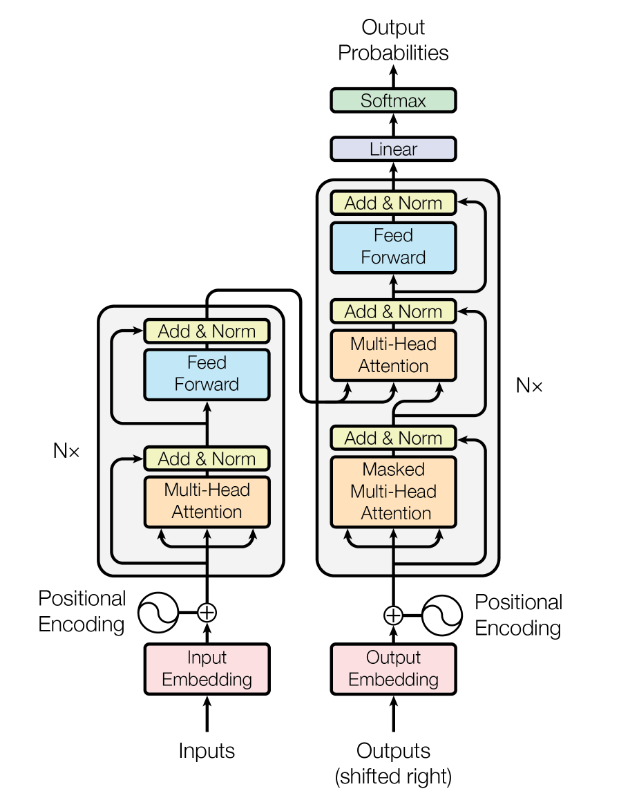
\includegraphics[width=0.6\textwidth]{images/transformers_architecture.png}
    \caption{Transformer Architecture with encoder (left) and decoder (right), Source: Vaswani \cite{vaswani2023attentionneed}}
    \label{fig:transformer_architecture}
\end{figure}

Figure \ref{fig:transformer_architecture} illustrates the Transformer architecture. Both encoder and decoder can be standalone models. Text must be tokenized through a dictionary to have a fixed size and frozen vocabulary.
The encoder embeds a sequence of tokens and passes them to the the positional encoding layer to preserve information for token position. Subsequently, it passes through multiple layers of multi-head self-attention and feed-forward neural network blocks. Attention heads compute token relevance via scaled dot-product
$softmax(QK^T/\sqrt{d_k})V$ where Q,K,V are learned projections. The outputs of the encoder is a real-valued numberical vector and can be passed to the decoder.
The decoder embeds an empty or predefined sequence. It gets passed to several layers of masked and non-masked multi-head self-attention, plus a feed forward neural network blocks. The mask ensures the decoder can only use preceding tokens. The output probabilities forecast the next token in sequence. Therefore prior decoder outputs can be used to autoregressively generate sequences of tokens.

% \paragraph{Encoder}

% The encoder transforms the sequences in a list of tokens and passes them to the input embedding layer and to the the positional encoding layer. Subsequently, it passes through multiple layers of multi-head self-attention and feed-forward neural network blocks. The outputs of the encoder is passed to the decoder, if the architecture is an encoder-decoder architecture. Encoders can also stand alone for tasks like text and code classification. (\citet{Hou.8212023})

% \paragraph{Decoder}

% In the encoder-decoder architecture the decoder begins with an initial output sequence or an empty sequence. The output sequence is passed to the output embedding layer and to the positional encoding layer. After that it gets passed to several layers of masked and non-masked multi-head self-attention, plus a feed forward neural network blocks. The outputs of the decoder is passed to the output layer, which is a linear layer followed by a softmax function. The output layer predicts the next token in the output sequence. The output sequence is passed to the decoder again, so that the model can predict the next token based on the previous tokens. This process is called autoregressive generation.
% The decoder can also stand-alone for autoregressive tasks like code completion, text to code generation, debugging, etc. as shown in \citet{Hou.8212023}.

% \paragraph{Input Embedding}
% Depending on the model, the input and output sequences are tokenized into subwords, words or characters. The input embedding layer converts tokenized sequences into dense vector representations. The input embedding layer is trained along with the rest of the model. The output of the input embedding layer is passed to the positional encoding layer. The positional encoding layer adds information about the position of each token in the input sequence, so that the model can distinguish between words with the same token but different positions. Positional encodings are combined with input embeddings before being fed into the encoder. The output embedding is equivalent to the input embedding, but it is used to convert the output tokens into a dense vector representation. The output embedding is used in the decoder part of the Transformer architecture.

% \paragraph{Multi-Head Self-Attention Block}

% Both in the encoder and in the decoder, a block consists of several multi-head self-attention layers followed by a feed-forward neural network layer. The multi-head self-attention layer is the main component of the Transformer architecture. It allows the model to weigh the importance of each token in the input sequence for each other token. The multi-head self-attention layer consists of multiple heads. Each head consists of a Query, Key and Value matrix, which are used to calculate the attention scores between the input tokens. The attention scores are used to weigh the importance of each token in the input sequence for each other token. The attention mechanism is mathematically defined as:

% $$Attention(Q,K, V) = softmax(\frac{QK^T}{\sqrt{d_k}})V$$

% Query (Q), Key (K) and Value (V) are matrices of the input tokens. This mechanism is based on common retrieval. Query can be seen as the search query, Key as the potential candidates and Value as the retrieved information.

% All matrices are learned during training. Query and Key are used to calculate the attention scores. The division by $\sqrt{d_k}$ is used to stabilize the gradients during training. The softmax function is used to normalize the attention scores. For the decoder part with the masked multi-head self-attention, the attention scores are masked with $-\infty$ for every token after the current calculated one right before the softmax, so that the model can only attend to previous tokens in the output sequence and the next predicted token is based only on the previous tokens. All attention heads are concatenated, passed through a linear layer, which is finally followed by a layer normalization to stabilize the gradients during training. 

% \paragraph{Putting it all together}
% After the input sequence is passed through the encoder, the output sequence is passed through the decoder. The decoder uses the encoder output as additional input and autoregressively predicts the next token in the output sequence. The output sequence is passed to the output layer, which is a linear layer followed by a softmax function. The output layer predicts the next token in the output sequence. The output sequence is passed to the decoder again, so that the model can predict the next token based on the previous tokens. This process is called autoregressive generation.

% There are several ways to predict the next token within the output layer. The most straightforward way is to predict the token with the highest probability. This is called greedy decoding. Another way is to sample the next token from the probability distribution. This is called sampling. There are also other ways to predict the next token, such as beam search, nucleus sampling, top-k sampling, top-p sampling, etc. These methods are used to improve the performance of the model. In the following the most important tuning parameters for LLMs are explained.

\subsection{Tuning Parameters}

There are several tuning parameters that can be used to improve the performance of LLMs. Some of the most important tuning parameters are:

\paragraph{Temperature}
The temperature parameter is used to control the randomness of the generated text. A high temperature value leads to more randomness, while a low temperature value leads to less randomness. The temperature parameter T modifies the softmax function as follows:

%include graphic
\begin{figure}[h!]
    \centering
    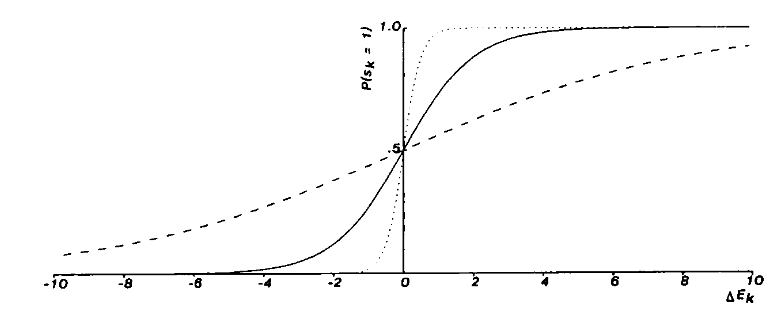
\includegraphics[width=0.6\textwidth]{images/temperature.png}
    \caption{The softmax function with different temperature values, T=1.0 (solid), T=4.0 (dashed), T=0.25 (dotted), Source: Ackey et al.\cite{ACKLEY.1985}}
    \label{fig:temperature}
\end{figure}

$$softmax: o(z)_i = \frac{e^{\beta z_i}}{\sum_{j=1}^K e^{\beta z_i}}$$

In figure \ref{fig:temperature} the softmax function is shown. A low temperature value leads to a peaky distribution, while a high temperature value leads to a more uniform distribution and therefore to more randomness.


% split paragraph in two parts
\paragraph{Top-K Sampling}
Top-K sampling \cite{Fan.13.05.2018} randomly selects from the top K tokens with the highest probability before applying the softmax function. Therefore the higher the K value, the more tokens are considered for sampling. Higher values increase output randomness. With Top-K equal to 1, the model behaves like greedy decoding.

\paragraph{Top-P Sampling}
The Top-P sampling \cite{Holtzman.22.04.2019} randomly selects from the smallest set of tokens whose cumulative probability exceeds the probability P. Therefore the higher the P value, the more tokens are considered for sampling. The outcomes gets more random. It is a generalization of Top-K sampling, where the number of tokens to sample from is not fixed.

\subsection{Prompting Techniques}
The Transformer architecture is not deterministic as shown in previous sections. Additionally LLMs have a high variance for its outputs too. The input prompt critically influences output quality. Therefore there are plenty of prompting techniques to stabilize desired outputs. Schulhoff created a taxonomy and recognized 58 LLM prompting techniques \cite{Schulhoff.06.06.2024}. I discuss four representative prompting techniques: Few-Shot, Zero-Shot, Chain-of-Thought (CoT), and Chain-of-Verification (CoVe). The list is not complete, but those are very commonly used and easy to implement.

\paragraph{Few-Shot vs. Zero-Shot}

\begin{figure}[h!]
    \centering
    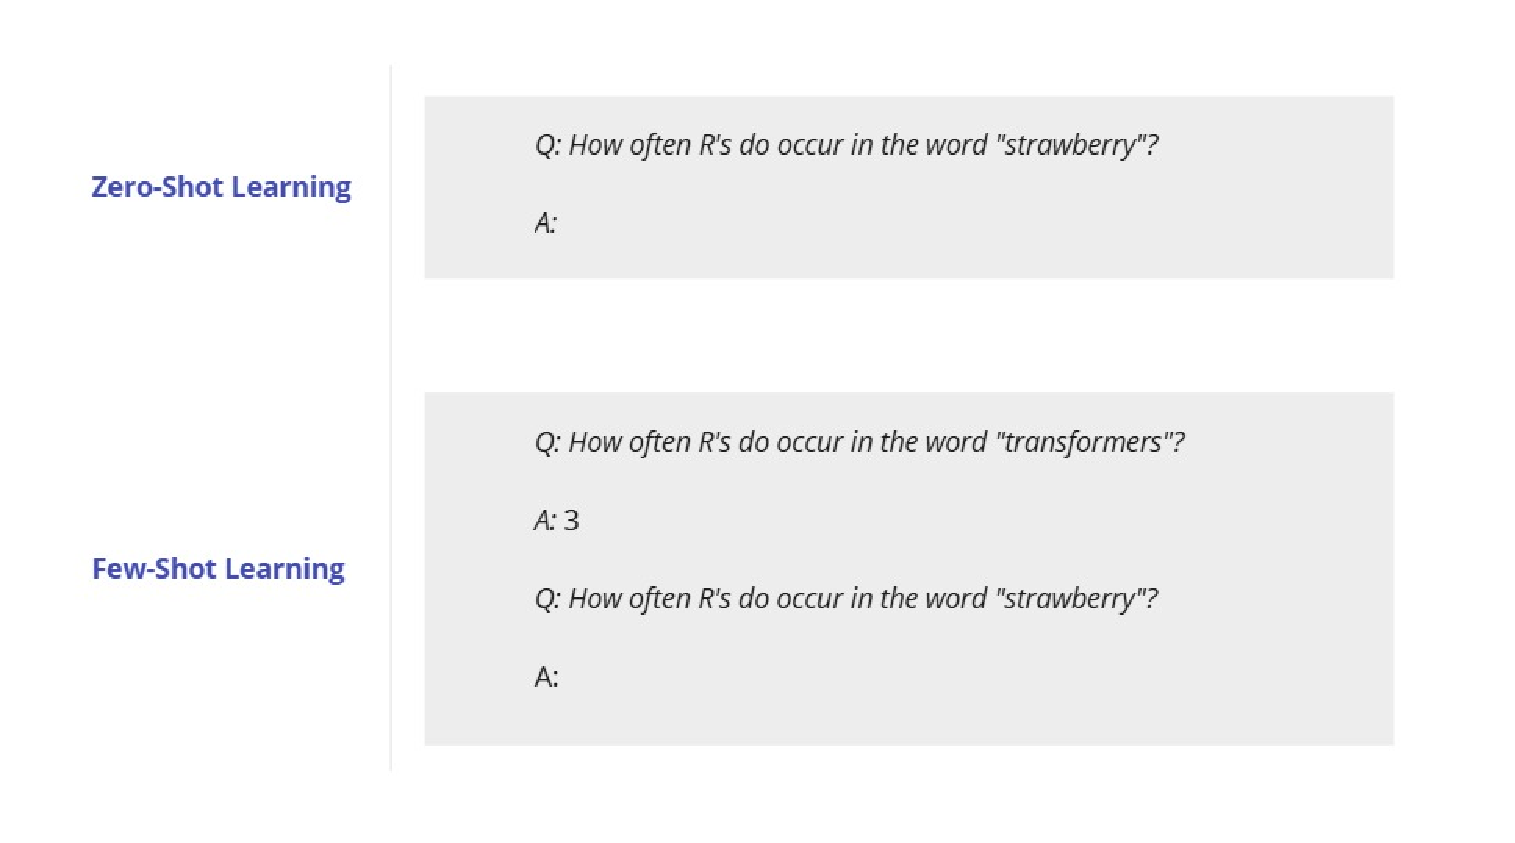
\includegraphics[width=\textwidth]{images/FewShot vs ZeroSHot.pdf}
    \caption{An example with a difficult query, that many LLM struggle, first without example (Zero-Shot) and below with one example (Few-Shot).}
    \label{fig:FewZeroShot}
\end{figure}


Few-Short prompting is a form of In-Context Learning (ICL), in which the prompt has examples of similar tasks to show the model how a task should be done. Brown showed that large models can leverage examples for various tasks \cite{Brown.28.05.2020}. Zero-Shot prompting refers then to prompting without showing examples before the task. Even though Few-Shot prompting might increase performance of LLMs, it comes with increased costs, as there are more tokens to process. An example of those prompting methods can be seen in figure \ref{fig:FewZeroShot}.

\paragraph{Chain-of-Thought}

\begin{figure}[h!]
    \centering
    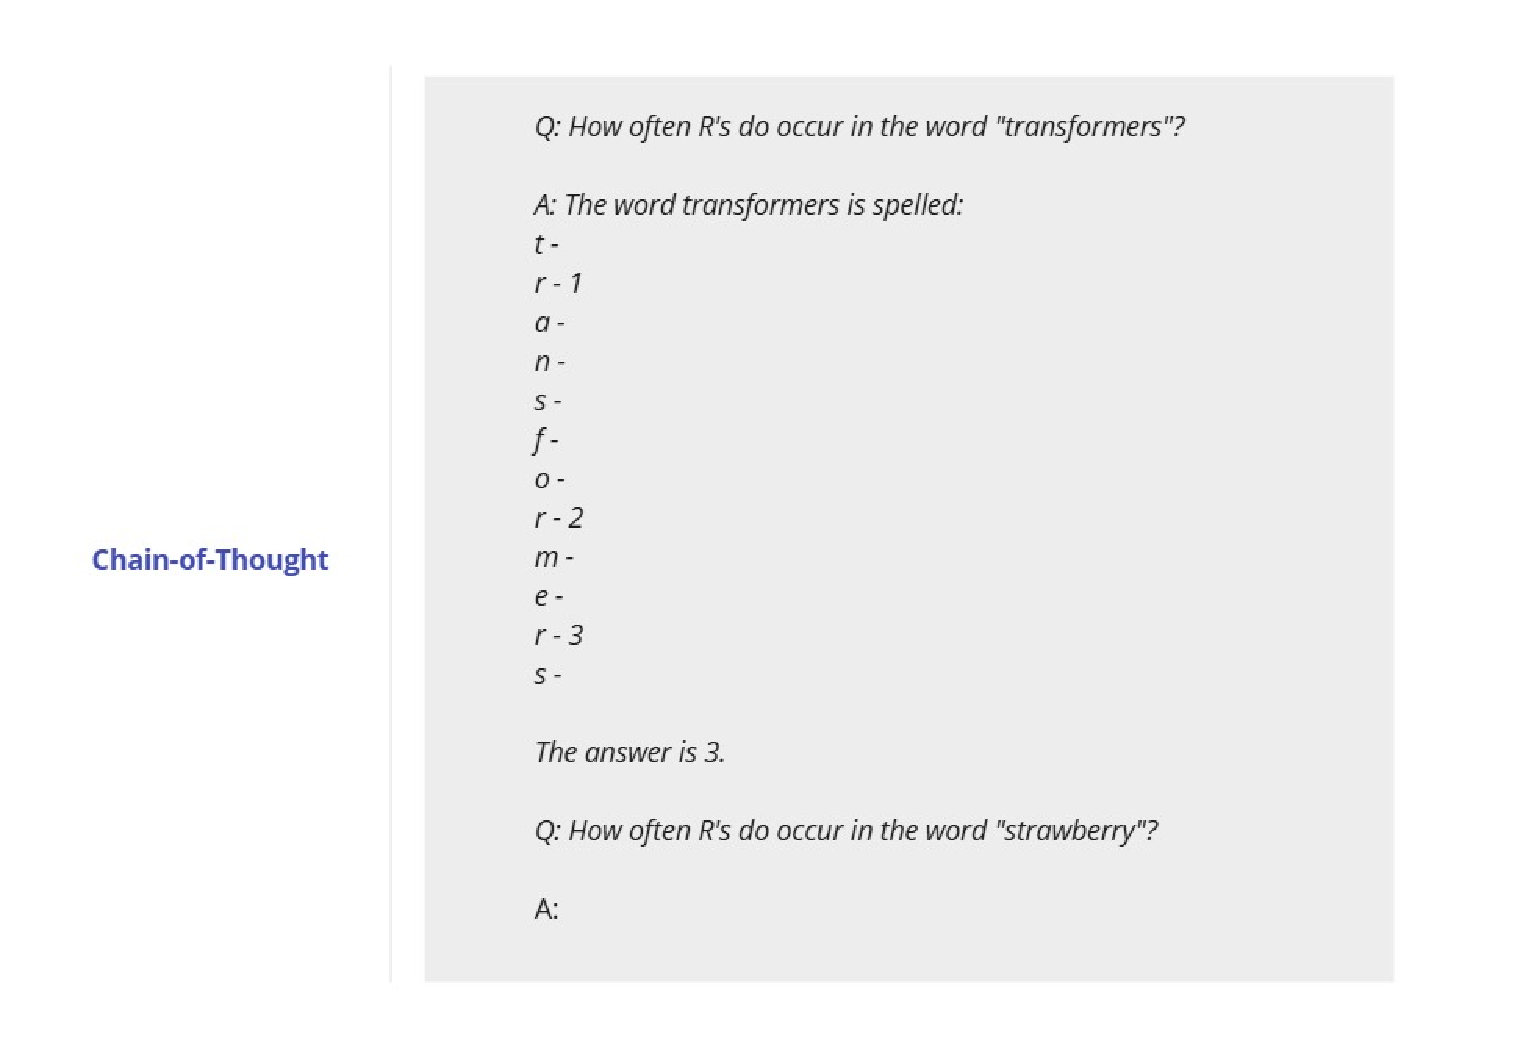
\includegraphics[width=\textwidth]{images/Chain-of-Thought.pdf}
    \caption{An Chain-of-Thought example with a difficult query, that many LLM struggle without prompting techniques}
    \label{fig:CoT}
\end{figure}


This method introduced by Wei leverages Few-Shot learning through simulating a written thought process in prior examples \cite{Wei.28.01.2022}. The LLM is therefore forced to take over this behaviour, which leads to more accurate outputs in reasoning and math problems. Schulhoff refers to it as the class of Thought Generation techniques \cite{Schulhoff.06.06.2024}. Figure \ref{fig:CoT} shows an example prompt.

\paragraph{Chain-of-Verification}
